\newpage
\subsection{Excluding certain projects from the export}

Sometimes it might be necessary to be able to exclude projects from the export (\texttt{Export All to Workspace} option).
This might be (i) because the project is still work in progress and simply not yet ready to be exported, (ii) because the complete project is present in your
Eclipse workspace but has not been modelled completely in EA and you wish to do this gradually on demand (this is currently the recommended strategy as we do
not have an import yet), (iii) because the project is not meant to be present in your Eclipse workspace as generated code and is instead provided via a plugin
(this is usually the case for standard metamodels like Ecore, UML etc.), or (iv) because the project is rather large and pretty stable, and you do not want to
wait each time for an unnecessary export (and you do not wish to click and export the other projects individually).
Whatever the reason, you can achieve this by setting a certain \emph{tagged value} of the project to be ignored:

\begin{enumerate}
\item[$\blacktriangleright$]Select ``View/Tagged Values'' from the menu bar (Fig.~\ref{fig_ignoreExportingProject01}).
\begin{figure}[htbp]
\begin{center}  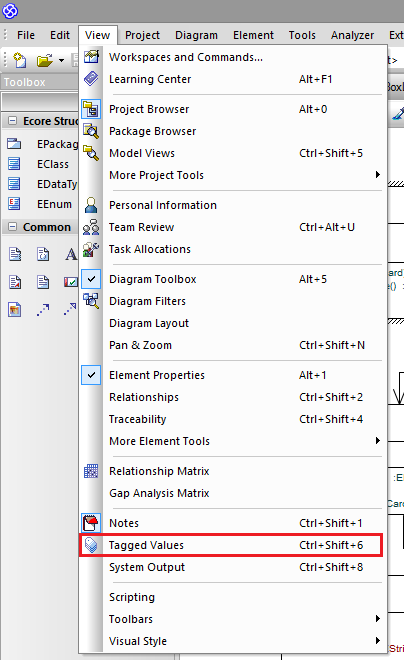
\includegraphics[width=0.55\textwidth]{ignoreExportingProject1}
  \caption{view the TaggedValue}  
  \label{fig_ignoreExportingProject01}
\end{center}
\end{figure} 

\item[$\blacktriangleright$] A tagged value \emph{Moflon::Export} should already be present and be set to \texttt{true} per default
(Fig.~\ref{fig_ignoreExportingProject02}). If this is not the case then create it afresh. If you want the project to be ignored by the export, change the value
of Moflon::Export to \texttt{false} (and conversely back to \texttt{true} to export it again).

\begin{figure}[htbp]
\begin{center}
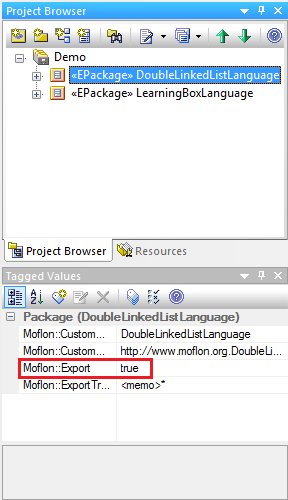
\includegraphics[width=0.5\textwidth]{ignoreExportingProject2}
  \caption{Tagged value Moflon::Export is used to ignore projects}  
  \label{fig_ignoreExportingProject02}
\end{center}
\end{figure}
\end{enumerate}